%%% Template originaly created by Karol Kozioł (mail@karol-koziol.net) and modified for ShareLaTeX use

\documentclass[a4paper,11pt,pagenumber=true]{article}

\usepackage{graphicx,url}
\usepackage[brazil]{babel}   
\usepackage[utf8]{inputenc}  
\usepackage{dirtytalk}
\usepackage{verbatim}
\usepackage{listings}
\usepackage{xcolor}

%\renewcommand\familydefault{\sfdefault}
%\usepackage{tgheros}
%\usepackage[defaultmono]{droidmono}

\usepackage{pifont,textcomp,gensymb}
\usepackage{amsmath,amssymb,amsthm}
\usepackage{enumerate, multicol}
\usepackage{tikz}

\usepackage{geometry}
\geometry{
    total={210mm,297mm},
    left=25mm,right=25mm,%
    bindingoffset=0mm, 
    top=20mm,bottom=20mm
}
\linespread{1.3}

\newcommand{\linia}{\rule{\linewidth}{0.5pt}}

% vectors specification shortcuts.
\newcommand{\vecu}{$\mathbf{u}$}
\newcommand{\vecv}{$\mathbf{v}$}
\newcommand{\vecw}{$\mathbf{w}$}
\newcommand{\vecp}{$\mathbf{p}$}
\newcommand{\vecq}{$\mathbf{q}$}
\newcommand{\veca}{$\mathbf{a}$}
\newcommand{\vecb}{$\mathbf{b}$}

% other math shortcuts. Use only on math mode.
\newcommand{\vecnorm}[1]{\|\mathbf{#1}\|}
\newcommand{\dotprod}[2]{\mathbf{#1} \bullet \mathbf{#2}}

\newtoks\institution

% custom theorems if needed
\newtheoremstyle{mytheor}
    {1ex}{1ex}{\normalfont}{0pt}{\scshape}{.}{1ex}
    {{\thmname{#1 }}{\thmnumber{#2}}{\thmnote{ (#3)}}}
\theoremstyle{mytheor}
\newtheorem{defi}{Definition}

% my own titles
\makeatletter
\renewcommand{\maketitle}{
    \begin{center}
        \vspace{2ex}
        {\huge \textsc{\@title}}
        \vspace{1ex}\\
        \linia\\
        \@author\\ 
        \linia\\
        \vspace{1ex}
        \textsc{\the\institution} 
        \hfill \@date
        \vspace{4ex}
    \end{center}
}
\makeatother
%%%

% custom footers and headers
\usepackage{fancyhdr}
\pagestyle{fancy}
\lhead{}
\chead{}
\rhead{}
\lfoot{Lista de Exercícios de Computação Gráfica \textnumero{1}}
\cfoot{}
\rfoot{Página \thepage}
\renewcommand{\headrulewidth}{0pt}
\renewcommand{\footrulewidth}{0pt}
%

% code listing settings
\usepackage{listings}
\renewcommand{\lstlistingname}{Listagem}
\renewcommand{\lstlistlistingname}{Relação de \lstlistingname s}
\lstset{
    language=R,
    basicstyle=\ttfamily\small,
    aboveskip={1.0\baselineskip},
    belowskip={1.0\baselineskip},
    columns=fixed,
    extendedchars=true,
    breaklines=true,
    tabsize=4,
    prebreak=\raisebox{0ex}[0ex][0ex]{\ensuremath{\hookleftarrow}},
    frame=lines,
    showtabs=false,
    showspaces=false,
    showstringspaces=false,
    keywordstyle=\color[rgb]{0.627,0.126,0.941},
    commentstyle=\color[rgb]{0.133,0.545,0.133},
    stringstyle=\color[rgb]{01,0,0},
    numbers=left,
    numberstyle=\small,
    stepnumber=1,
    numbersep=10pt,
    captionpos=t,
    escapeinside={\%*}{*)},
    literate={á}{{\'a}}1 {â}{{\^a}}1 {ã}{{\~a}}1 {à}{{\`a}}1 {é}{{\'e}}1 {ê}{{\^e}}1 {ó}{{\'o}}1 {ô}{{\^o}}1 {õ}{{\~o}}1 {ú}{{\'u}}1 {~}{{\~}}1 {é}{{\'e}}1 {ç}{{\,c}}1 {í}{{\'i}}1
}

%%%----------%%%----------%%%----------%%%----------%%%

\begin{document}

    \title{Lista de Exercícios de\\Computação Gráfica \textnumero{1}}

    \author{Jonas de Araújo Luz Jr.\\
    unifor@jonasluz.com}
    \institution{Profa. Andreia Formico}
    \date{04/03/2017}
    
    \begin{figure}[t]
    \centering
        
\includegraphics[width=.2\textwidth]{images/logo-UNIFOR.jpg}
        \label{fig:logo}    
    \end{figure}
    
    \maketitle
    \tableofcontents
    \newpage
    
    \section{Especificação}

        \begin{figure}[h]
        \centering
            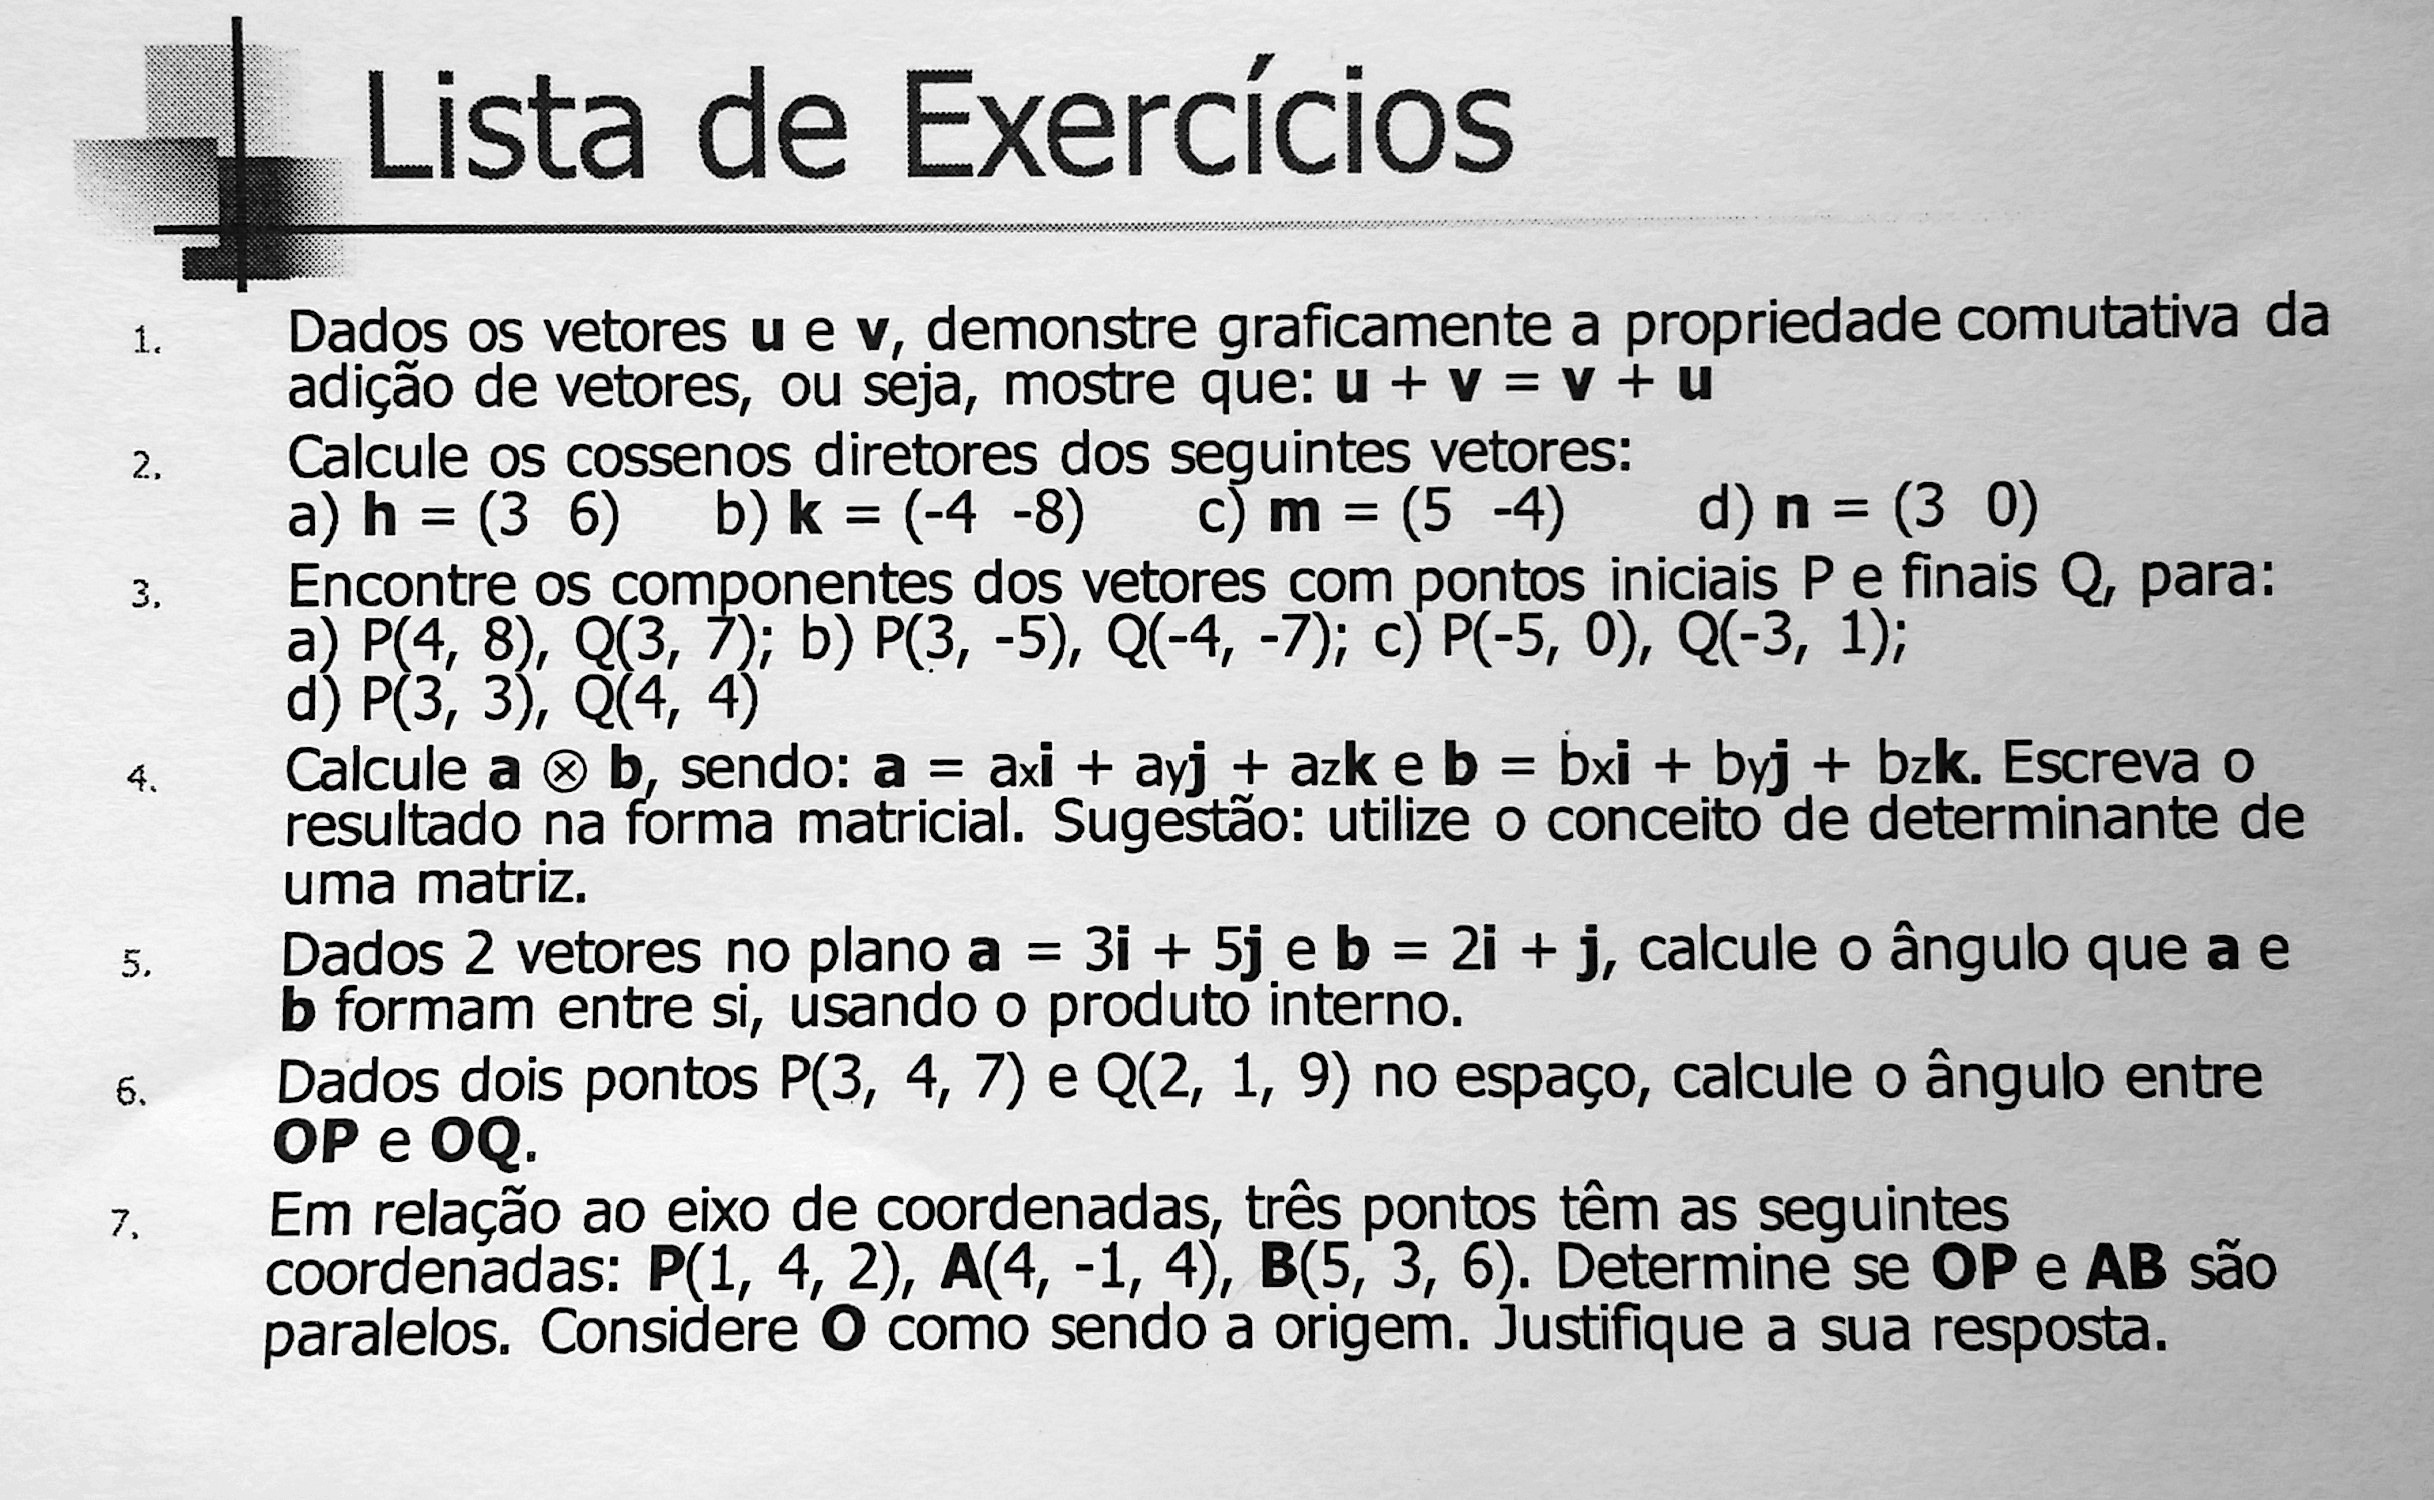
\includegraphics[width=1\textwidth]{images/Especificacao-1.jpg}
            \label{fig:spec1}    
        \end{figure}
        \begin{figure}[h]
        \centering
            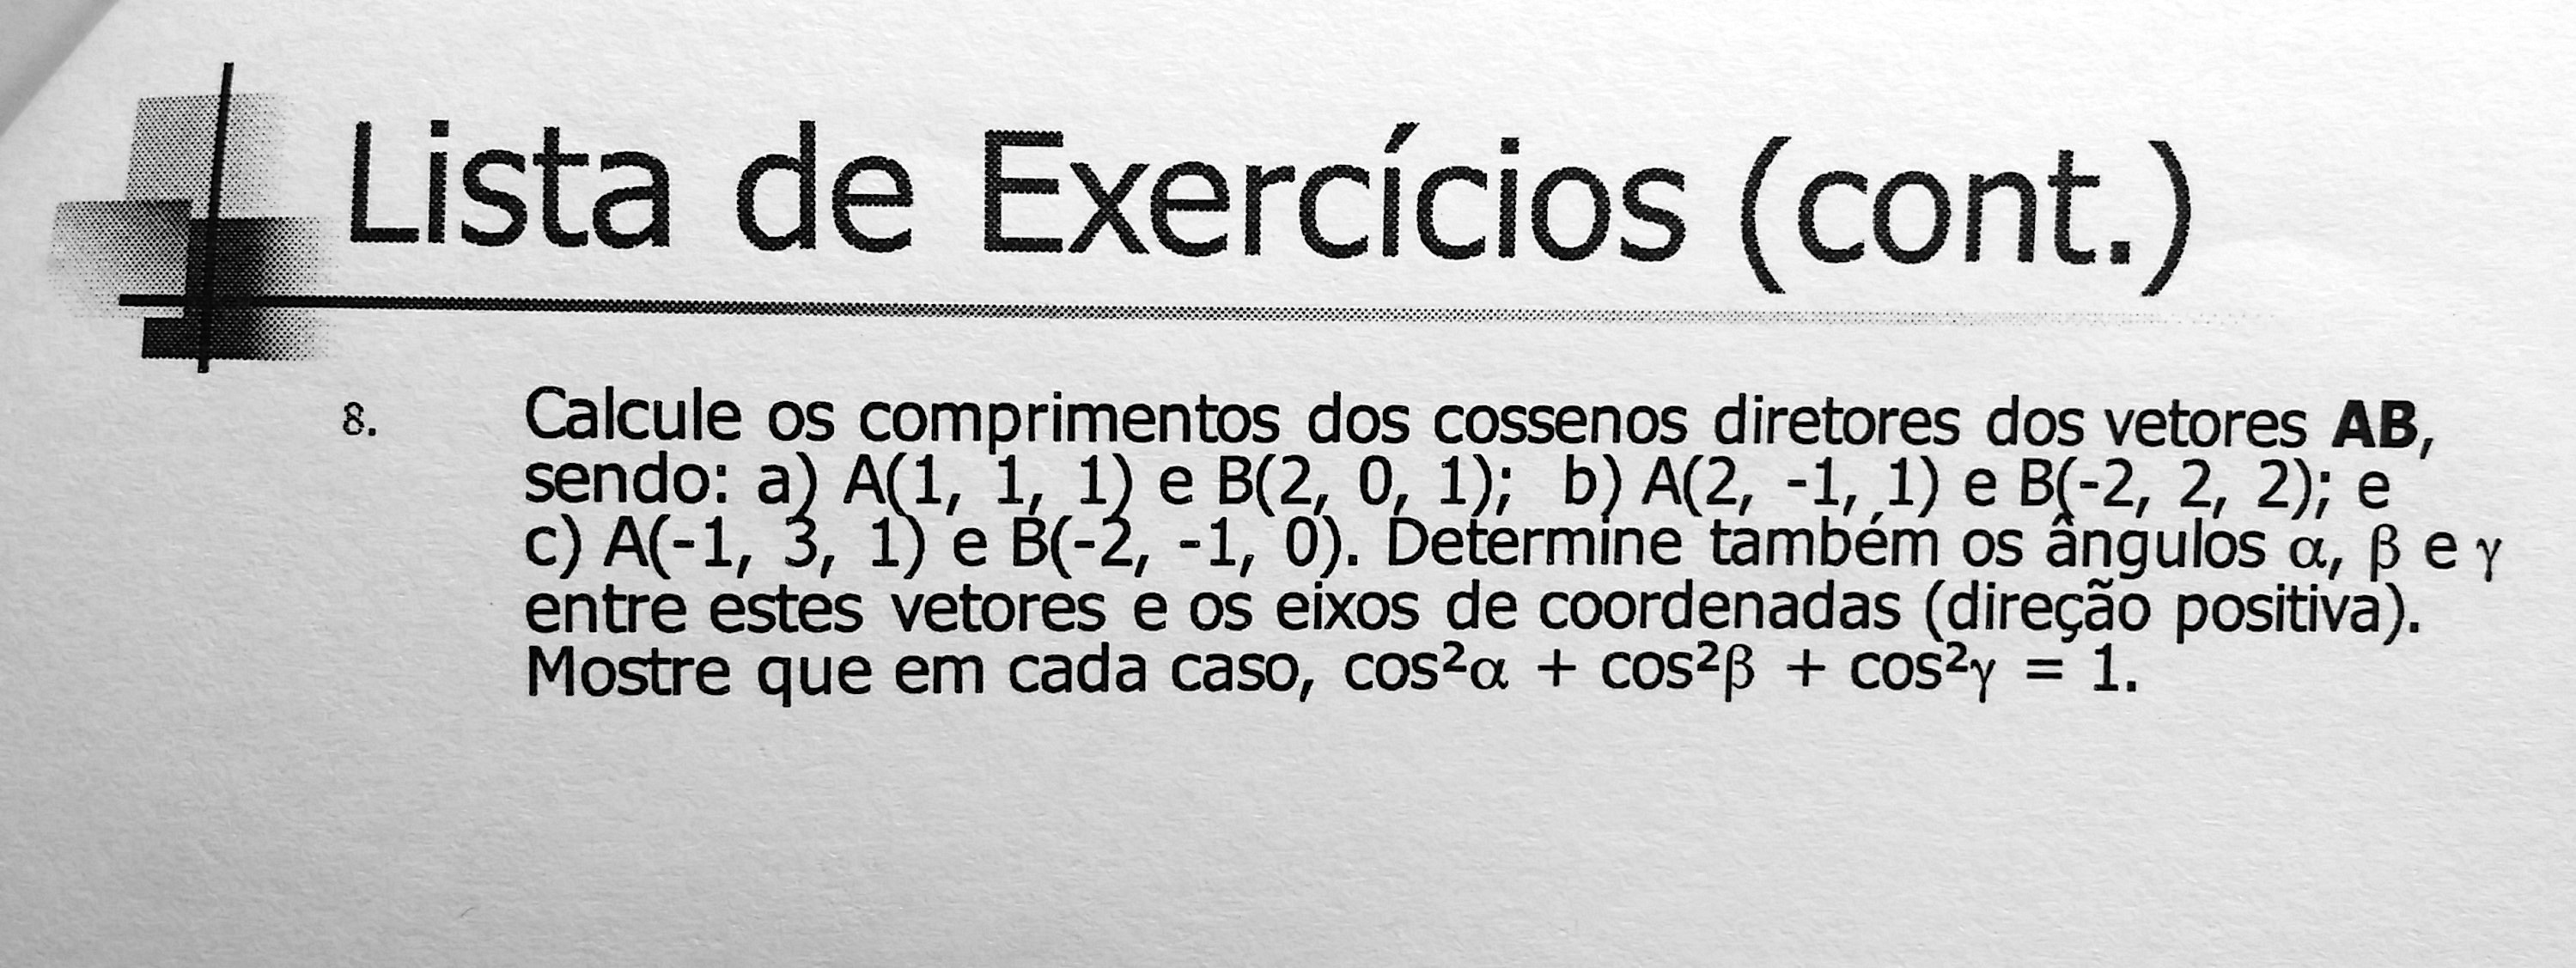
\includegraphics[width=1\textwidth]{images/Especificacao-2.jpg}
            \label{fig:spec2}    
        \end{figure}

    \newpage
    
    \section{Soluções}
    
        \subsection{Questão \textnumero{1}}
        % Question 1
            
            Sejam os vetores \vecu{} e \vecv{} genéricos, simbolizados na Figura \ref{fig:q1-1}.

            \begin{figure}[h]
            \centering
                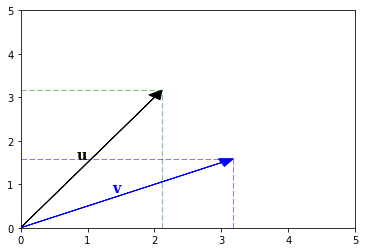
\includegraphics[width=.5\textwidth]{images/q1-1.png}
                \caption{Vetores \vecu{} e \vecv{} quaisquer.}
                \label{fig:q1-1}    
            \end{figure}
            
            Fazendo \vecv{} partir de \vecu, temos \vecu+\vecv, mostrado na Figura \ref{fig:q1-2}
            
            \begin{figure}[h]
            \centering
               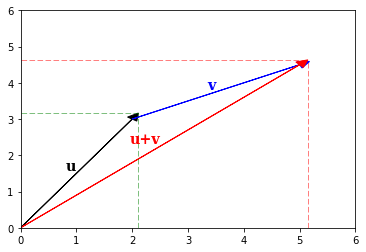
\includegraphics[width=.5\textwidth]{images/q1-2.png}
                \caption{Vetor \vecu+\vecv.}
                \label{fig:q1-2}    
            \end{figure}
            
            Agora, para obter \vecv+\vecu, fazemos \vecu{} partir de \vecv, o que é mostrado na Figura \ref{fig:q1-3}.
        
            \begin{figure}[h]
            \centering
               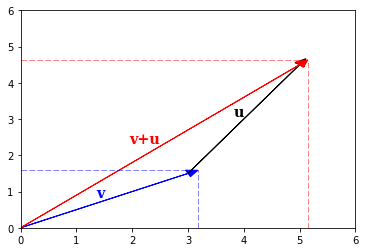
\includegraphics[width=.5\textwidth]{images/q1-3.png}
                \caption{Vetor \vecv+\vecu.}
                \label{fig:q1-3}    
            \end{figure}
            
            Vê-se que os vetores resultantes \vecu+\vecv{} e \vecv+\vecu{} são idênticos. A Figura \ref{fig:q1-4} ilustra ambos, evidenciando que estão sobrepostos.
            
             \begin{figure}[h]
            \centering
               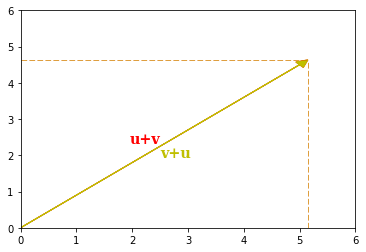
\includegraphics[width=.5\textwidth]{images/q1-4.png}
                \caption{Vetor \vecu+\vecv.}
                \label{fig:q1-4}    
            \end{figure}
        
        \clearpage
    
        \subsection{Questão \textnumero{2}}
        % Question 2
        
            Para dado vetor \vecv{} com componentes $c_1, c_2, \dotsc, c_n$, ou seja,
            $\mathbf{v} = [c_1, c_2, \dotsc, c_n]$, o cosseno diretor $\cos \alpha_k$ para cada componente $c_k$ é dado por: 
            
            \begin{equation}\label{eq:dcos}
                \cos \alpha_k = \frac{c_k}{\vecnorm{v}}
            \end{equation}
            
            onde $\vecnorm{v}$ é a \textit{norma} do vetor \vecv, dada por:
            
            \begin{equation}\label{eq_norm}
                \vecnorm{v} = \sqrt{c_1^2 + c_2^2 + \dotsb + c_n^2}
            \end{equation}
            
            % 2.a)
            \subsubsection*{a) $\mathbf{h} = [3, 6]$}
            \[ \vecnorm{h} = \sqrt{3^2 + 6^2} = \sqrt{9 + 36} = \sqrt{45} = 3 \sqrt{5} \]
            \[ \cos \alpha_x = \frac{3}{3 \sqrt{5}} = \frac{1}{\sqrt{5}} = \mathbf{0.4472} \]
            \[ \cos \alpha_y = \frac{6}{3 \sqrt{5}} = \frac{2}{\sqrt{5}} = \mathbf{0.8944} \]
            
            % 2.b)
            \subsubsection*{b) $\mathbf{k} = [-4, 8]$}
            \[ \vecnorm{k} = \sqrt{(-4)^2 + 8^2} = \sqrt{16 + 64} = \sqrt{80} = 4 \sqrt{5} \]
            \[ \cos \alpha_x = \frac{-4}{4 \sqrt{5}} = \frac{-1}{\sqrt{5}} = \mathbf{0.4472} \]
            \[ \cos \alpha_y = \frac{8}{4 \sqrt{5}} = \frac{2}{\sqrt{5}} = \mathbf{0.8944} \]

            % 2.c)
            \subsubsection*{c) $\mathbf{m} = [5, -4]$}
            \[ \vecnorm{m} = \sqrt{5^2 + (-4)^2} = \sqrt{25 + 16} = \sqrt{41} \]
            \[ \cos \alpha_x = \frac{5}{\sqrt{41}} = \mathbf{0.7809} \]
            \[ \cos \alpha_y = \frac{-4}{\sqrt{41}} = \mathbf{0.6247} \]

            % 2.d)
            \subsubsection*{d) $\mathbf{n} = [3, 0]$}
            \[ \vecnorm{n} = \sqrt{3^2 + 0^2} = \sqrt{9 + 0} = \sqrt{9} = 3\]
            \[ \cos \alpha_x = \frac{3}{3} = \mathbf{1} \]
            \[ \cos \alpha_y = \frac{0}{3} = \mathbf{0} \]
                
        \clearpage
        
        \subsection{Questão \textnumero{3}}
        % Question 3
        
            Para cada ponto $P(x_p, y_p)$ e $Q(x_q, y_q)$, o vetor \vecv{} iniciado em $P$ e terminado em $Q$ é dado por $\mathbf{q}-\mathbf{p}$ onde \vecp{} corresponde ao vetor que sai da origem do eixo de coordenadas e termina em $P$, e \vecq{} corresponde ao vetor que sai da origem do eixo de coordenadas e termina em $Q$.\\
            
            Desta forma, temos que \vecv{} é dado por $\mathbf{v} = [x_q-x_p, y_q-y_p]$.
            
            % 3.a)
            \subsubsection*{a) $P(4, 8), Q(3, 7)$}
            \[\mathbf{v} = [3-4, 7-8] = \mathbf{[-1, -1]}\]
            
            % 3.b)
            \subsubsection*{b) $P(3, -5), Q(-4, -7)$}
            \[\mathbf{v} = [-4-3, -7-(-5)] = \mathbf{[-7, -2]}\]
            
            % 3.c)
            \subsubsection*{c) $P(-5, 0), Q(-3, 1)$}
            \[\mathbf{v} = [-3-(-5), 1-0] = \mathbf{[2, 1]}\]
            
            % 3.d)
            \subsubsection*{d) $P(3, 3), Q(4, 4)$}
            \[\mathbf{v} = [4-3, 4-3] = \mathbf{[1, 1]}\]

        \subsection{Questão \textnumero{4}}
        % Question 4
        
            O produto vetorial de dois vetores 
            $\mathbf{a} = a_x\mathbf{i} + a_y\mathbf{j} + a_z\mathbf{k}$ e 
            $\mathbf{b} = b_x\mathbf{i} + b_y\mathbf{j} + b_z\mathbf{k}$ é definido pela fórmula
            
            \begin{equation}\label{eq:cross-product}
                \mathbf{a}\times\mathbf{b} = 
                    (a_y b_z - a_z b_y)\mathbf{i} + 
                    (a_z b_x - a_x b_z)\mathbf{j} + 
                    (a_x b_y - a_y b_x)\mathbf{k}                 
            \end{equation}
    
            a qual corresponde ao determinante da matriz quadrada 
            \(  \begin{bmatrix}
                    i       & j     & k     \\
                    a_x     & a_y   & a_z   \\
                    b_x     & b_y   & b_z 
                \end{bmatrix}
            \). Ou seja:
            
            \begin{equation}\label{eq:cross-detmat}
                \mathbf{a}\times\mathbf{b} = 
                \begin{vmatrix}
                    i       & j     & k     \\
                    a_x     & a_y   & a_z   \\
                    b_x     & b_y   & b_z 
                \end{vmatrix}                
            \end{equation}
            
            Portanto, podemos reescrever a Equação \ref{eq:cross-product} como produto de uma matriz linha por uma coluna, tal que: 
            
            \begin{equation}\label{cross-matrix}
                \begin{split}
                    \mathbf{a}\times\mathbf{b} = 
                    \begin{bmatrix}
                        a_y b_z - a_z b_y   && a_z b_x - a_x b_z    && a_x b_y - a_y b_x
                    \end{bmatrix}_{1,3} \cdot 
                    \begin{bmatrix}
                        \mathbf{i} \\ 
                        \mathbf{j} \\ 
                        \mathbf{k}
                    \end{bmatrix}_{3,1} \\ =
                    \begin{bmatrix}
                        (a_y b_z - a_z b_y)\mathbf{i} +
                        (a_z b_x - a_x b_z)\mathbf{j} +
                        (a_x b_y - a_y b_x)\mathbf{k}
                    \end{bmatrix}_{1,1}
                \end{split}
            \end{equation}
            o que resulta em uma matriz $1\times1$, cujo único valor -- que corresponde ao valor de seu
            determinante -- é dado pela mesma Equação \ref{eq:cross-product}.

        \subsection{Questão \textnumero{5}}
        % Question 5
        
            O produto interno entre dois vetores de mesma dimensão $n$, 
            $\mathbf{a} = \langle a_1, a_2, \dotsc, a_n \rangle$ e
            $\mathbf{b} = \langle b_1, b_2, \dotsc, b_n \rangle$ é um escalar definido por:
            
            \begin{equation}\label{eq:dotprod-1}
                \dotprod{a}{b} = a_1 b_1 + a_2 b_2 + \dotsb + a_n b_n
            \end{equation}
            
            O produto interno entre os dois vetores \veca{} e \vecb{} também pode ser obtido pela fórmula
            
            \begin{equation}\label{eq:dotprod-2}
                \dotprod{a}{b} = \vecnorm{a} \vecnorm{b} \cos \theta
            \end{equation} onde $\theta$ é o ângulo formado entre \veca{} e \vecb{}.
            
            Desta forma, conhecendo-se os vetores \veca{} e \vecb{}, e após se determinar o valor do 
            produto interno por meio da Equação \ref{eq:dotprod-1}, pode-se calcular o valor de $\theta$ como sendo: 
            
            \begin{equation}\label{internal-angle}
                \theta = \arccos \left(\frac{\dotprod{a}{b}}{\vecnorm{a}\vecnorm{b}}\right)
            \end{equation} \\
            
            Para os vetores $\mathbf{a} = 3\mathbf{i} + 5\mathbf{j}$ e 
            $\mathbf{b} = 2\mathbf{i} + \mathbf{j}$, temos:
            
            \[\dotprod{a}{b} = 3\times2 + 5\times1 = 6 + 5 = 11\]
            \[\vecnorm{a} = \sqrt{3^2 + 5^2} = \sqrt{9 + 25} = \sqrt{34}\] 
            \[\vecnorm{b} = \sqrt{2^2 + 1^2} = \sqrt{4 + 1} = \sqrt{5}\].
            
            Daí, obtemos que: 
        
            \[
                \theta_{\mathbf{a},\mathbf{b}} = \arccos \left(\frac{11}{\sqrt{34}\sqrt{5}}\right) =
                \arccos(0.84366) = \mathbf{32.471192\degree}
            \]
            
        \subsection{Questão \textnumero{6}}
        % Question 6
        
            Os segmentos de reta $OP$ e $OQ$, sendo o ponto $O$ a origem, $P(3, 4, 7)$ e $Q(2, 1, 9)$,
            correspondem, respectivamente, aos vetores 
            $\mathbf{p}\langle 3, 4, 7 \rangle$ e $\mathbf{q} \langle 2, 1, 9 \rangle$.
            Desta forma o ângulo entre $OP$ e $OQ$ corresponde ao ângulo entre os vetores 
            \vecp{} e \vecq{} e pode ser obtido por meio da Equação \ref{eq:dotprod-2}. 
            
            Para os vetores \vecp{} e \vecq{} dados, da Equação \ref{eq:dotprod-1}, temos que:
            \[\dotprod{p}{q} = 3 \times 2 + 4 \times 1 + 7 \times 9 = 6 + 4 + 63 = 73\]
            \[\vecnorm{p} = \sqrt{3^2 + 4^2 + 7^2} = \sqrt{9 + 16 + 49} = \sqrt{74}\]
            \[\vecnorm{q} = \sqrt{2^2 + 1^2 + 9^2} = \sqrt{4 + 1 + 81} = \sqrt{86}\]
            
            Daí:
            
            \[
                \theta_{\mathbf{p},\mathbf{q}} = \arccos \left(\frac{73}{\sqrt{74}\sqrt{86}}\right) =
                \arccos(0.915077) = \mathbf{23.783295\degree}
            \]
        
        \subsection{Questão \textnumero{7}}
        % Question 7
        
            Sendo os pontos $P(1, 4, 2)$, $A(4, -1, 4)$ e $B(5, 3, 6)$ e $O$ a origem, os segmentos de reta
            $OP$ e $AB$ correspondem, respectivamente, aos vetores $\mathbf{p} \langle 1, 4, 2 \rangle$ e
            $\mathbf{q} = \mathbf{b} \langle 5, 3, 6 \rangle - \mathbf{a} \langle 4, -1, 4 \rangle$, que 
            resulta, este último, no vetor $\mathbf{q} \langle 1, 4, 2 \rangle$, o qual, constata-se, é
            igual a \vecp, ou seja \textbf{\vecp{} e \vecq{} são coincidentes e, portanto, paralelos}. \\
            
            Outra forma de demonstrar o paralelismo dos vetores \vecp{} e \vecq{} é por meio do ângulo $\theta$ formado entre eles que, sendo os vetores paralelos, deve ser igual a zero e, neste caso, $cos \theta_{p,q} = 1$. Fazendo uso das Equações \ref{eq:dotprod-1} e \ref{eq:dotprod-2} podemos verificar isto. Inicialmente, temos que: 
            
            \[\dotprod{p}{q} = 1 \times 1 + 4 \times 4 + 2 \times 2 = 1 + 16 + 4 = 21\]
            \[\vecnorm{p} = \sqrt{1^2 + 4^2 + 2^2} = \sqrt{1 + 16 + 4} = \sqrt{21}\]
            \[\vecnorm{q} = \sqrt{1^2 + 4^2 + 2^2} = \sqrt{1 + 16 + 4} = \sqrt{21}\]

            E daí: 
            
            \[
                \theta_{\mathbf{p},\mathbf{q}} = 
                    \arccos \left(\frac{21}{\sqrt{21 \times 21}}\right) =
                    \arccos(1) = \mathbf{0}
            \]
            
            o que comprova que \vecp{} e \vecq{} \textbf{são paralelos}.
        
        \subsection{Questão \textnumero{8}}
        % Question 8
        
            Para cada par de pontos $A$ e $B$, o vetor $AB$ é dado por 
            $\mathbf{v} = \langle x_b - x_a, y_b - y_a, z_b - z_a \rangle$. 
            
            Por sua vez, os cossenos diretores do vetor são dados pela Equação \ref{eq:dcos}.
            
            \subsubsection*{a) $A(1,1,1)$ e $B(2,0,1)$}
                
                $\mathbf{v} = \langle 2 - 1, 0 - 1, 1 - 1 \rangle = \langle 1, -1, 0 \rangle$
                
                \[ \vecnorm{v} = \sqrt{1^2 + (-1)^2 + 0^2} = \sqrt{2} \]
                
                Os cossenos diretores são:
                
                \[ \cos \alpha = \frac{1}{\sqrt{2}}  = \mathbf{0.7071} \]
                \[ \cos \beta  = \frac{-1}{\sqrt{2}} = \mathbf{-0.7071} \]
                \[ \cos \gamma = \frac{0}{\sqrt{2}}  = \mathbf{0} \]
        
                Destes, se obtêm os ângulos $\alpha$, $\beta$ e $\gamma$, por meio do arco-cosseno:
                
                \[\alpha = \arccos 0.7071  = \mathbf{45\degree}\]
                \[\beta  = \arccos -0.7071 = \mathbf{135\degree}\]
                \[\gamma = \arccos 0       = \mathbf{90\degree}\]
                
                E, agora, pode-se verificar que:
                
                \[ 
                    \cos^2 \alpha + \cos^2 \beta + \cos^2 \gamma = 
                    (0.7071)^2 + (-0.7071)^2 + 0^2 = \mathbf{1}
                \] conforme se queria demonstrar.
                
           \subsubsection*{b) $A(2,-1,1)$ e $B(-2,2,2)$}
                
                $\mathbf{v} = \langle -2 - 2, 2 + 1, 2 - 1 \rangle = \langle -4, 3, 1 \rangle$
                
                \[ \vecnorm{v} = \sqrt{(-4)^2 + 3^2 + 1^2} = \sqrt{26} \]
                
                Os cossenos diretores são:
                
                \[ \cos \alpha = \frac{-4}{\sqrt{26}}  = \mathbf{-0.7845} \]
                \[ \cos \beta  = \frac{3}{\sqrt{26}} = \mathbf{0.5883} \]
                \[ \cos \gamma = \frac{1}{\sqrt{26}}  = \mathbf{0.1961} \]
        
                Disto:
                
                \[\alpha = \arccos -0.7845 = \mathbf{141.671\degree}\]
                \[\beta  = \arccos 0.5883  = \mathbf{53.9601\degree}\]
                \[\gamma = \arccos 0.1961  = \mathbf{78.6901\degree}\]
                
                E agora: 
                
                \[ 
                    \cos^2 \alpha + \cos^2 \beta + \cos^2 \gamma = 
                    (-0.7845)^2 + (0.5883)^2 + (0.1961)^2 = \mathbf{1}
                \] conforme se queria demonstrar.        
                
           \subsubsection*{c) $A(-1,3,1)$ e $B(-2,-1,0)$}
                
                $\mathbf{v} = \langle -2 + 1, -1 - 3, 0 - 1 \rangle = \langle -1, -4, -1 \rangle$
                
                \[ \vecnorm{v} = \sqrt{(-1)^2 + (-4)^2 + (-1)^2} = \sqrt{18} = 2\sqrt{3} \]
                
                Os cossenos diretores são:
                
                \[ \cos \alpha = \frac{-1}{2\sqrt{3}}  = \mathbf{-0.2357} \]
                \[ \cos \beta  = \frac{-4}{2\sqrt{3}} = \mathbf{-0.9428} \]
                \[ \cos \gamma = \frac{-1}{2\sqrt{3}}  = \mathbf{-0.2357} \]
        
                Então:
                
                \[\alpha = \arccos -0.2357 = \mathbf{103.633\degree}\]
                \[\beta  = \arccos -0.9428 = \mathbf{160.529\degree}\]
                \[\gamma = \arccos -0.2357 = \mathbf{103.633\degree}\]
                
                E, por fim: 
                
                \[ 
                    \cos^2 \alpha + \cos^2 \beta + \cos^2 \gamma = 
                    (-0.2357)^2 + (-0.9428)^2 + (-0.2357)^2 = \mathbf{1}
                \] conforme se queria demonstrar. $\Box$
    
\nocite{*}
\bibliographystyle{acm}
\bibliography{assignment}

\end{document}
